% В этом шаблоне используется класс spbau-diploma. Его можно найти и, если требуется,
% поправить в файле spbau-diploma.cls
\documentclass{spbau-diploma}
\begin{document}
% Год, город, название университета и факультета предопределены,
% но можно и поменять.
% Если англоязычная титульная страница не нужна, то ее можно просто удалить.
\filltitle{ru}{
    chair              = {Кафедра математических и информационных технологий},
    title              = {Генерация зависимых языков по спецификации пользователя},
    % Здесь указывается тип работы. Возможные значения:
    %   coursework - Курсовая работа
    %   diploma - Диплом специалиста
    %   master - Диплом магистра
    %   bachelor - Диплом бакалавра
    type               = {master},
    position           = {студента},
    group              = 604,
    author             = {Гарифуллин Шамиль Раифович},
    supervisorPosition = {аспирант},
    supervisor         = {Исаев В.\,И.},
    reviewerPosition   = {аспирант},
    reviewer           = {Подкопаев А.\,В.},
    chairHeadPosition  = {д.\,ф.-м.\,н., профессор},
    chairHead          = {Омельченко А.\,В.},
    % university = {САНКТ-ПЕТЕРБУРГСКИЙ АКАДЕМИЧЕСКИЙ УНИВЕРСИТЕТ},
    % faculty = {Центр высшего образования},
    % city = {Санкт-Петербург},
    % year             = {2013}
}
\filltitle{en}{
    chair              = {Department of Mathematics and Information Technology},
    title              = {Specification based generation of languages with dependent types},
    author             = {Shamil Garifullin},
    supervisorPosition = {PhD student},
    supervisor         = {Valeriy Isaev},
    reviewerPosition   = {PhD student},
    reviewer           = {Anton Podkopaev},
    chairHeadPosition  = {professor},
    chairHead          = {Alexander Omelchenko},
}
\maketitle
\tableofcontents

\section*{Введение}
Теории зависимых типов были впервые введены Мартин-Лёфом в семидесятых годах прошлого века\cite{early_lof}, затем была написана книга~\cite{martin_lof}. Одна из основных его мотиваций заключалась в том, чтобы предложить альтернативу теории множеств для формализации математики. Сама теория типов обладает рядом преимуществ перед теорией множеств (описаны в статье~\cite{farmer_seven}, а преимущества теорий зависимых типов описаны в \cite{shulman_homotopy}), благодаря которым формализация математики становится проще.

% О теории типов можно также думать как о типизированном функциональном языке программирования. Существует множество различных языков, основанных на теориях зависимых типов.

Наиболее известными примерами языков с зависимыми типами, которые используются для доказательства математических утверждений являются Coq\cite{coq} и Agda\cite{agda}. Например, доказательство теоремы о четырех красках было завершено в 2005 году с помощью Coq\cite{weisstein2002four}.

Другая область применения теорий зависимых типов --- это верификация программ. Так как использование произвольных выражений языка на уровне типов значительно расширяет экспрессивность системы типов языка, можно задавать произвольные ограничения на входные и выходные данные функций языка. Таким способом можно описывать и формально верифицировать даже большие системы, например существует формально верифицированная версия Standard ML\cite{ml_lang} под названием CakeML\cite{ml_cake}. Пример относительно простой верификации --- корректности функции filter на Agda приведен в Приложении~\ref{sort_proof}.

\hfill

При реализации языков с зависимыми типами возникает ряд типичных задач, основной из которых является реализация функции проверки типов. Однако для eё реализации необходимо реализовывать функцию вычисления выражений и проверки их на равенство, для этого необходимо уметь совершать манипуляции с выражениями языка --- а значит их тоже реализовывать (подробнее про реализацию в подразделе про реализацию и Разделе~\ref{impl_section}). Цель данной работы заключается в том, чтобы реализовать приложение, которое по спецификации зависимого языка (подробнее о языке спицификации в Разделе~\ref{lang_spec}) генерирует исходный код на каком-либо языке (для этих целей мы используем Haskell\cite{haskell}), осуществляющий проверку типов заданного языка.

С одной стороны такое приложение упростит реализацию языков с зависимыми типами, так как, благодаря ему, можно будет избежать реализации фактически шаблонного кода. С другой стороны, позволит эксперементировать с различными вариациями теорий типов для более близкого знакомства с ними.

Поэтому основной задачей данной работы является определение языка спецификации зависимых языков, с дальнейшей генерацией представления АСД этого языка и функций работы с деревом в виде модуля Haskell\cite{haskell}. \textit{АСД} --- абстрактное синтаксическое дерево, по любому выражению языка можно составить дерево, узлами этого дерева будут конструкции языка, а потомками узла выражения к которым конструкция применяется. Генерируемый модуль содержит функции проверки типов, вычисления выражений, работы с контекстами и стандартных операций над выражениями (такие как подстановка, абстракция и проверка на равенство).

Текст работы состоит из трёх основных разделов. Каждый из них мы обсудим подробнее в соответствующем подразделе введения.

\subsection*{Языки с зависимыми типами}

Все зависимые языки состоят из некоторых конструкций языка, с помощью которых затем пишутся все выражения в языке.

Например, язык булевых выражений Bool состоит из четырёх конструкций: тип Bool, константы true и false, и конструкция if-then-else. Нас интересуют только типизированные языки, поэтому для каждой конструкции должны быть прописаны правила типизации. В нашем языке true имеет тип Bool, false имеет тип Bool, if-then-else принимает четыре аргумента --- выражение типа Bool, тип возвращаемого выражения и два выражения, имеющих тип равный возвращаемому.

Также необходимо задавать правила вычисления языка, их принято называть правилами \textit{редукции} языка. Для Bool их всего два, а именно для конструкции if-then-else мы возвращаем либо ветку then, либо ветку else в зависимости от первого её аргумента.

Такое описание языка достаточно неформально, как языки задаются через формальные правила вывода см. Разделы~\ref{deptypes_intro}~и~\ref{lang_spec}.

Выше был представлен пример обычного, независимого языка Bool. Чтобы из него сделать зависимый язык Bool, нужно модифицировать конструкцию if-then-else, чтобы она могла принимать зависимые типы. Теперь вторым её аргументом будет функция, возвращающая тип возвращаемого выражения в зависимости от переданного ей аргумента типа Bool --- тип зависит от выражения языка, переданного в него. Тогда станет возможной конструкция вида: if-then-else(t, f, True, 1), которая будет возвращать либо True типа Bool, либо 1 типа Int в зависимости от истинности первого аргумента конструкции. Более подробное введение в зависимые языки можно найти в~\cite{martin_lof}.

\subsection*{Определение языка спецификаций}

Наша цель научиться записывать правила типизации формально и по такому описанию генерировать код, который бы осуществлял проверку типов для соответствующего языка.

Формализация языка происходит путем описания его спецификации. В спецификации задаются возможные уровни выражений языка, например в Haskell это типы, термы и виды. Затем описываются его конструкции --- для них объявляются уровни аргументов и возвращаемого выражения. Также задаются правила типизации каждой конструкции и правила редукции языка.

Затем описание проходит проверку на корректность (определение языка спецификации и проверки описаны в Разделе~\ref{lang_spec}). Эта проверка должна исключать как просто некорректно записанные языки, так и языки для которых генерация кода будет проблематичной или невозможной. Поэтому важной частью этой подзадачи является огрничение множества языков, которые возможно специфицировать в нашем языке.

Стоит отметить, что спецификация позволяет задавать нестабильные теории (см. Раздел~\ref{lang_spec} для более подробного описания). Это ограничение полезно для определенных теоретических применений теории типов, которые мы не будем обсуждать в данной работе, так как они выходят за её рамки. Одним из применений нестабильности является формализация~\cite{ncat:inf}.

% Например, если мы хотим, чтобы конструкцию if-then-else можно было применять только, если все свободные переменные внутри неё имеют тип Bool или являются функциями из Bool в Bool, мы можем проаннотировать соответствующее правило вывода списком типов $[Bool, Bool\rightarrow Bool]$.

\subsection*{Реализация}

После проверок спецификации (описанных в Разделе~\ref{constraints}) строится структура хранящая информацию о правилах вывода, редукциях и конструкциях языка. С её помощью происходит кодогенерация представления выражений языка и функций проверки типов и вычисления.

В дальнейшем мы понимаем вычисление как переписывание выражений согласно редукциям языка, пока не получим выражение к которому ни одна редукция неприменима --- этот процесс называется приведением выражения в \textit{нормальную форму}.

Нормализация генерируется по правилам редукции, описанным в спецификации, функция проверки типов --- по правилам вывода. Неявно подразумевается, что в языке есть отношение эквивалентности на выражениях, которое порождается отношением редукции. Это выражается в том, что сравнение выражений (которое сравнивает их с точностью до этого отношения эквивалентности) сначала нормализует выражения, а потом сравнивает их нормальные формы.

Так как типы зависимого языка могут включать в себя произвольные выражения, проверка типов является задачей тесно связанной с вычислением языка. Например, если наша функция принимает только списки длинны числа фибоначчи, а нам передана конкатенация списков длины 2 и 3 то, чтобы понять является ли это число числом фибоначчи, нам нужно его вычислить $2 + 3 => 5$, также вычислить первые несколько чисел фибоначчи, положим числа фибоначчи определены как список $[1,1,2,3,5,8,...]$, затем вычислить предикат принадлежности $5 \in fibs$, и только тогда мы можем вызвать функцию сравнения выражений. Также стоить заметить, что выражения могут иметь достаточно сложную нормальную форму и нам может прийтись сравнивать АСД этих выражений.

Поэтому написание функции проверки типов языка становится достаточно ёмкой задачей --- мы должны попутно реализовывать функцию нормализации. Однако общий алгоритм проверки типов не сильно отличается от языка к языку --- всегда нужно рекурсивно проверять АСД на удовлетворение правилам вывода, таким образом его можно генерировать по спецификации, при наличии достаточного количества ограничений на последнюю (подробнее в Разделе~\ref{typecheck}).


Как упоминалось выше, правильно выбранное представление может значительно упростить генерацию кода. Также существуют варианты представления, дающие больше гарантий на корректность составления выражений языка, благодаря более строгой типизации. Рассмотрены несколько вариантов представления (см. Раздел~\ref{term_repr} для подробного обсуждения этих вариантов):
\begin{enumerate}
\item Обычное именованное (переменные представляются в виде строк)
\item Обычные индексы де Брейна\cite{de_brujin} (переменные явяются целыми числами, указывающими на место их связывания)
\item Индексы де Брейна с использованием полиморфной рекурсии\cite{poly_rec}
\end{enumerate}

У первых двух способов представления есть недостатки. В первом необходимо вводить $\alpha$-эквивалентность на выражениях --- \textit{$\alpha$-эквивалентными} называются выражения, которые отличаются только в именовании связанных переменных. Также в каждом из этих случаев легко допустить ошибку при работе с выражениями. Третий вариант является модификацией второго, в которой совершать ошибки при работе с индексами сложнее из-за проверок на уровне типов, таким образом код пользователя получается имеет больше гарантий корректности.

В дополнение, третий подход позволяет с большей легкостью генерировать операции над выражениями: равенство проверяется непосредственно, подстановки и абстракция тоже не составляют больших усилий.





%%


\section{Постановка задачи}

Целью данной работы является дизайн и имплементация языка для спецификации языков программирования с зависимыми типами. Ключевые задачи, которые решает работа:
\begin{itemize}
  \item Сужение множества возможных спецификаций зависимых языков для возможности генерации тайпчекера.
  \item Реализация генерации структур данных представления языка и функций манипуляции этими структурами.
  \item Реализация генерации функций приведения термов специфицированного языка в нормальную форму и проверки типов.
\end{itemize}

\section{Зависимые языки} \label{deptypes_intro}
Во многих языках программирования возникают ошибки связанные с доступом за границу массива.
Аналогом этого в Haskell является взятие первого элемента в списке.

\begin{lstlisting}[frame=single]
head :: [a] -> a
head (x:_) = x
head [] = error "No head!"
\end{lstlisting}

Такие ситуациях обычно решаются с помощью механизма исключений или его аналогов. Однако эту проблему можно решить иначе, наложив на вход дополнительные ограничения. А именно --- не принимать некорректные входные данные.

\begin{lstlisting}[frame=single]
head :: {n : N} -> Vec a (suc n) -> a
head (x:_) = x
\end{lstlisting}

Здесь тип явно специфицирует, что функция не принимает термы типа `Vec a 0'. Языки с зависимыми типами позволяют типам зависеть от термов, именно это позволяет описать тип списков фиксированной длины.

Как правило, программисты все равно проверяют какие-то ограничения перед вызовом функции или обладают дополнительной информацией, на основе которой они пишут код так, как они его пишут. В зависимых языках мы можем писать программы, где передача этого знания будет явно требоваться компилятором, что позволяет не допускать такого рода ошибки.

Этот способ обобщается, и можно доказывать корректность работы алгоритмов, например функции filter в Приложении~\ref{sort_proof}.

\subsection{Проверка типов в зависимых языках}\label{typecheck}
Рассмотрим пример правила вывода:

\begin{center}
\AxiomC{$\Gamma, x : S \vdash T\ type $}
\AxiomC{$\Gamma, \vdash f : \Pi(S, T) $}
\AxiomC{$\Gamma \vdash t : S $}
\TrinaryInfC{$\Gamma \vdash app(T, f, t) : T[x:=t]$}
\DisplayProof
\end{center}

Это пример правила вывода применения зависимой функции. $\Pi$ принимает в качестве аргумента терм и в зависимости от аргумента возвращает тип, обычные функции через $\Pi$ выражаются просто --- они всегда возвращают один и тот же тип.

Правила вывода можно представлять как узлы дерева вывода, где заключение является предком всех предпослок. Проверка типов в любом языке это обход АСТ и происходит так: мы имеем некоторые аргументы внутри примитива, которые мы используем для составления узлов-потомков (предпосылок). На этих узлах вызываем функцию вывода типов в возможно расширенном контексте\footnote{Конечно, мы должны для каждого расширения контекста проверять его корректность.} рекурсивно. Если потомки составлены корректно, то получаем некие типы, которые можем использовать в проверке равенств в предпосылках и возрате типа примитива.

В зависимых языках все точно так же, однако проверка на равенство должна происходить после нормализации термов. Нормализацию мы применяем только после того как убедимся, что термы корректно составлены. Получается, что нормализация тесно связана с проверкой типов. Более того проверка типов невозможна без нормализации термов.

Давайте разберём алгоритм на примере выше.
\begin{enumerate}
\item Чтобы проверить терм $app(T, f, t)$ (и вернуть его тип $T[x:=t]$), поочередно проверяем предпосылки. \item Вызываемся рекурсивно на терме $t$ и, если не произошло ошибки, получаем тип $S$.
\item Расширяем контекст типом $S$ и проверяем ``тип'' $T$ (на самом деле мы проверяем тип $T$ на определенность).
\item Вызываемся рекурсивно на $f$ --- получаем его тип. Теперь нужно проверить его на равенство типу $\Pi(S, T)$, который мы строим из имеющихся метапеременных. Подразумевается равенство нормальных форм. Соответственно равенство должно быть вызвано на нормализованных типах.
\item Если мы дошли до этой стадии, значит все определено корректно и мы возвращаем тип $T[x:=t]$
\end{enumerate}

Можно заметить, что мы должны уметь корректно выполнять подстановки и проверять термы на равенство, равенство подразумевается до $\alpha$-эквивалентности.

\subsection{Индексы де Брейна}\label{de_brujin}
При реализации функциональных языков одной из сложных проблем встающих перед программистом является выбор представления. Также нужно описывать подстановки\footnote{В работе подразумевается реализация языков программирования через описание AST на Haskell.} и многие проблемы и ошибки в реализации связаны с подстановками.

Одной из проблем представления термов является сравнение $\alpha$-эквивалентных термов. \textit{$\alpha$-эквивалентными} называются термы, которые отличаются только в именовании связанных переменных. Например, следующие три терма $\alpha$-эквивалентны:

\begin{lstlisting}
lamb x y → y (x z)
lamb y x → x (y z)
lamb a b → b (a z)
\end{lstlisting}

Одним из возможных способов представления термов является представление переменных в виде строк. С использованием такого подхода первый приведенный выше терм записывается в виде \lstinline{[Lam ``x'' (Lam ``y'' (App ``y'' (App ``x'' ``z'')))]}. Проверка равенства этого терма второму терму \lstinline{[Lam ``y'' (Lam ``x'' (App ``x'' (App ``y'' ``z'')))]} не тривиальна.

Другой проблемой такого представления термов является захвата свободных переменных при подстановке. Предположим, мы подставляем первый терм ниже в переменную ``z'' во втором.
\begin{lstlisting}
lamb x → y
lamb y → z
lamb y → lamb x → y = lamb y x → y
\end{lstlisting}

Очевидно, что подставлять в переменную так наивно нельзя, так как ``y'' стала связанной, хотя не была таковой в первоначальном терме.

Ключевым замечанием является то, что переменные в функциональных языках являются ``указателями'' на место их связывания --- этаким индексом в контекст --- и не несут никакой дополнительной информации.

Результат использования этого наблюдения называется индексами де Брейна. А именно: для каждой связанной переменной мы просто пишем расстояние от неё до ближайшего связывания.

Если переписать термы с альфа эквивалентностью выше, то для всех трех термов получим \lstinline{[lamb lamb → 1 (2 z)]}, и проверка на альфа-эквивалентность превращается в проверку на равенство.

Также решается проблема избегания захвата переменных, а именно:
\begin{lstlisting}
lamb → y
lamb → z
lamb → lamb → y = lamb lamb → y
\end{lstlisting}

Как видно ``y'' остался свободным.

Это представление значительно лучше удовлетворяет нашим требованиям разработчика языков. Мы перешли от
\lstinline{[Lam ``y'' (Lam ``x'' (App ``x'' (App ``y'' ``z'')))]} к \lstinline{[Lam (Lam (App 1 (App 2 ``z'')))]}.

Однако общей проблемой обоих представлений является нетипизированность переменных --- никто не контролирует построение термов вида \lstinline{[Lam (Lam (App 123 (App 23 ``z'')))]}. Решение этой проблемы описано в секции~\ref{de_brujin_impl}.









%--

\section{Обзор аналогов}
Построение языков программирования с зависимыми типами по спецификации является задачей достаточно специфичной. Ниже перечислены некотороые инструменты, применяемые в похожих ситуациях (изучение формальных систем, языков программирования и их реализация).

\subsection{BNFC}
Похожим на программу описанную в дипломной работе средством разработки является BNFC\cite{bnfc}. Эта утилита позволяет генерировать фронтенд компилятора по аннотированной грамматике языка в форме Бэкуса-Наура\cite{lbnf}.

Программа генерирует лексический анализатор, синтаксический анализатор и вывод структур на экран языка заданного в спецификации. Также она генерирует абстрактное синтаксическое дерево и заготовку для написания редукций, представленную в виде большой конструкции switch или её аналогов.

Генерирует представления на C, C++, C\#, Haskell, Java и OCaml.

\subsection{PLT/Redex}
PLT/Redex\cite{plt:redex} --- встроенный DSL на языке Racket, созданный для спецификации и изучения операционных семантик языков программирования. Используется для спецификации языков программирования, в том числе и с зависимыми типами.

Из отличительных черт: позволяет случайным образом тестировать цикличность редукций или иные свойства языка, задаваемые пользователем в DSL. Также позволяет визуализировать порядок редукций.

Однако спецификация языков с зависимыми типами занимает столько же усилий, как если бы пользователь писал реализацию языка в Haskell\cite{plt:ex}. Большую сложность составляют подстановки --- проблема, обойденная в данной дипломной работе благодаря использованию представления термов языка в виде индексов де Брейна.

\subsection{Twelf}
Twelf\cite{twelf} является реализацией LF\cite{Pfenning2002}. Используется для спецификации и доказательств свойств логик и языков программирования.

В спецификации задаются высказывания языка (используется принцип "высказывания в качестве типов"\cite{harper:1993}) и некоторые операции над ним в виде отношений на языке Twelf. Затем доказываются свойства вида  $\forall\Sigma$ специфицированного языка.

Таким образом, в Twelf можно доказывать свойства спецификаций языков или приводить спецификации к форме, в которой выполняются интересующие нас, как дизайнер, свойства. Затем можно использовать программу описанную в данной дипломной работе для реализации языка.






%--

\section{Определение языка спецификаций}\label{lang_spec}

Вдохновением данной работы послужила статьи~\cite{Palmgren} и~\cite{isaev}. Поэтому сам язык спецификации выглядит как язык описания алгебраических теорий\footnote{А именно: помимо правил вывода у нас есть сорта и функциональные символы.}.

Начнем с примера описания языка с зависимыми типами~(рис.\ref{lpi})~\cite[Глава~2.1]{book:pierce}

\begin{figure}
    \centering
	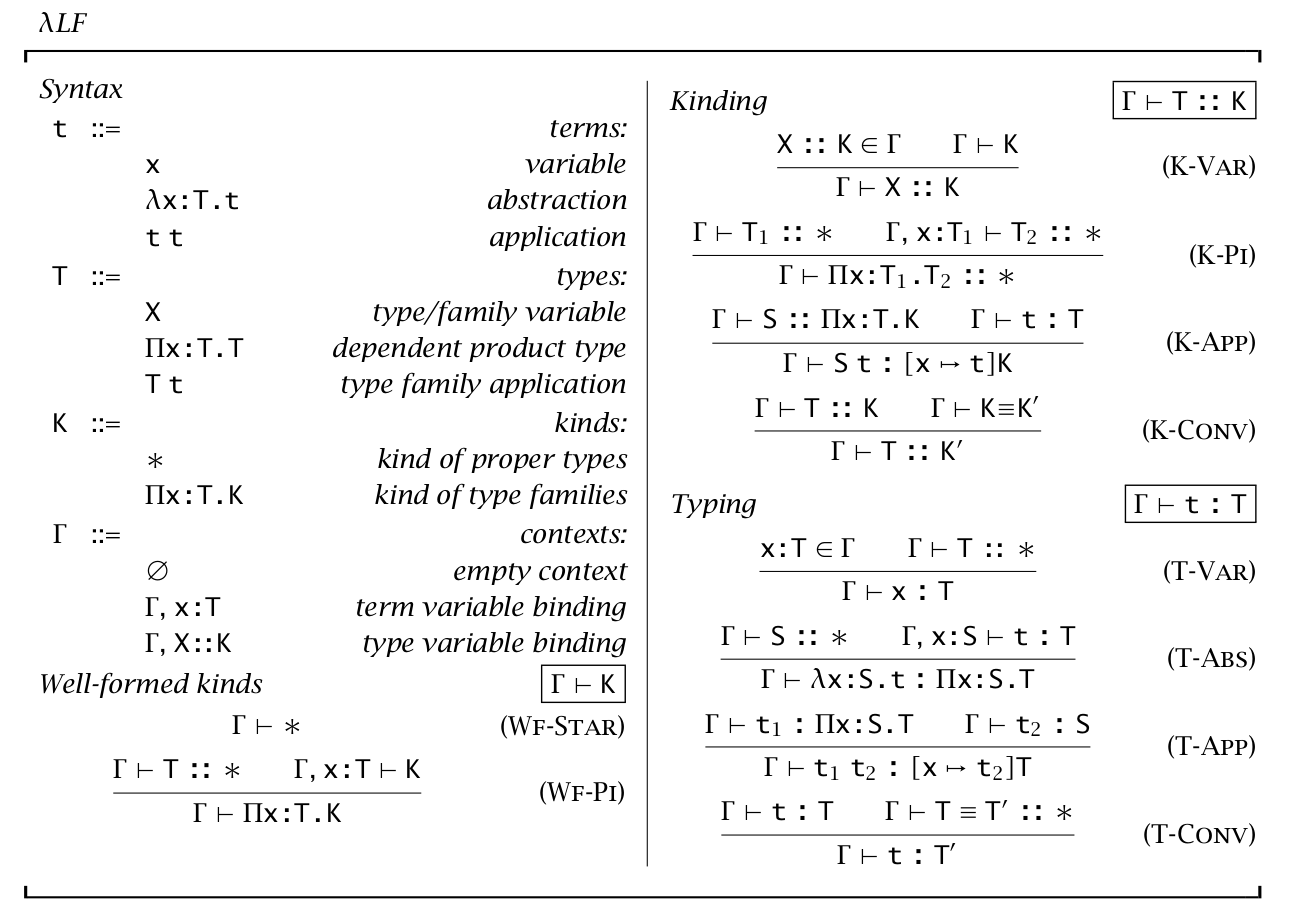
\includegraphics[scale=0.35]{img/lp.png}
	\caption{Язык с лямбдой и $\Pi$-типами }
	\label{lpi}
\end{figure}

У нас явно выделяются три сорта(можно думать о сортах как о метатипах): кайнды, термы и типы(правила связанные с кайндами и само их описание опущены для простоты).

Также явно выделяются примитивы языка\footnote{В дальнейшем мы называем из функциональными символами.}:
абстракция, пи-типы (стрелки в языках без зависимых типов) и аппликация. Легко заметить, что во всех яхыках присутствуют подстановка, контексты, символ ':' означающий что тип терма слева есть терм справа и связывание переменных.

Если принять во внимания все наблюдения выше то так этот язык будет выглядеть в нашем языке спецификации\footnote{Важно понимать что запись $\_ \vdash$ не означает что контекст пуст, если слева ничего не написано это эквивалентно записи $\Gamma \vdash$.}:

\begin{lstlisting}
DependentSorts:
  tm, ty
FunctionalSymbols:
  lam: (ty, 0)*(tm, 1) -> tm
  app: (tm, 0)*(tm, 0)*(ty, 1) -> tm
  pi : (ty, 0)*(ty, 1) -> ty
Axioms:
  K-Pi =
    forall T1 : ty, x.T2 : ty
      x : T1 |- T2 def |--- |- pi(T1, x.T2) def

  TAbs =
    forall S : ty, x.T : ty, x.t : tm
      x : S |- t : T |--- |- lam(S, x.t) : pi(S, x.T)
  TApp =
    forall t1 : tm, t2 : tm, S : ty, x.T : ty
            |- t1 : pi(S, x.T),
            |- t2 : S,
      x : S |- T def
      |--------------------------
      |- app(t1, t2, x.T) : T[x:=t2]
Reductions:
  Beta =
    forall x.b : tm, A : ty, a : tm, z.T : ty
       |--- |- app(lam(A, x.b), a, z.T) => b[x:=a] : T[z:=a]

\end{lstlisting}

Типизирование метапеременных позволяет проверять правильность применения функциональных символов и наличие нужных переменных в контексте. Именованные переменные служат для определения порядка переменных в контексте и не несут какой-то дополнительной информации.

Также в язык была добавлена проверка на c-стабильность - можно помечать аксиомы типами, тогда аксиома применима только если все переменные входящие в терм являются представителями этих типов\footnote{Если список типов пуст, то производится проверка на отсутствие свободных переменных}.

\subsection{Ограничения на спецификации, налагаемые языком}

\begin{enumerate}

\item Все используемые метапеременные должны иметь аннотацию (сорт), то есть присутствовать в секции forall аксиомы/редукции.

\item Запрещено равенство в заключении аксиом, для определенности каждого шага в проверке типов определяемого языка (если видим равенство не ясно в какую сторону идти при редуцировании)

\item Все аргументы в функциональный символ в заключении аксиомы должны быть метапеременными. Ещё и с теми же аргуементами что и в forall (не больше).

\item Если в заключении аксиомы написан функциональный символ возвращающий сорт, он обязан также иметь тип (нельзя просто написать $ \vdash f(\ldots) def$).

\item Определения функциональных символов всегда одно, иначе появляется недетерминированность в проверке типов. Не играет особой роли, тк в данном случае можно сделать недетерминированность в проверке.

\item Подстановки разрешены только в метапеременные - в принципе это слабое ограничение, которое облегчает жизнь при реализации, не ограничивая пользователя.

\item В заключении контекст не должен быть расширен - это ограничение связано с тем, что иначе смысл аксиомы становится странным. А именно: функциональный символ применим только при введении перепенных в контекст.

\item \label{tm:Meta} Все метапеременные используемые в предпосылках должны либо присутствовать в метапеременных заключения или же должны быть типами какой-либо предпосылки.

\item Если в функциональном символе встречаются метапеременные с контекстами $x_1 \ldots x_k . T$, должна существовать предпосылка вида $x_1 : S_1 \ldots x_k : S_k  \vdash T$. Это сделано для того чтобы не передавать типы контекстов метапеременных функционального символа явно.

\item Если метапеременная является типом предпосылки и не встречается в аргументах функционального символа, то она может использоваться только справа от двоеточия. Таким образом избегаются ситуации связанные с порядком проверки предпосылок языка. А именно: если у нас есть $x : S \vdash t : T, x:T \vdash r : S$. То нужно строить граф зависимостей для предпосылок и использовать порядок полученный в результате его топологической сортировки в генерации кода. (Аналогично с~\ref{toposort}).

\item \label{order:Meta} Все переменные контекстов метапеременных могут использовать только метапеременные левее внутри функционального символа в заключении - это связано с тем, что иначе могут возникнуть циклы в определениях метапеременных: S тип с аргументом типа R, R тип с аргументом типа S, S тип с аргументом типа R...

\item Из-за ослабления условия на метапеременные в Пункте~\ref{tm:Meta}, порядок метапеременных неочевиден. Решение данной проблемы и~(\ref{order:Meta}) описано в Секции~\ref{toposort}.

\item Редукции не учитывают предпосылок при приведении в нормальную форму - предполагается что они не конфликтуют с аксиомами и проверки в аксиомах достаточно.

\item В редукциях все метапеременные справа от '=>' должны встречаться и слева от него.

\item Подстановка запрещена слева от '=>'.

\item Все редукции всегда стабильны.

\end{enumerate}

\subsection{Проверки корректности спецификации языка}

Все ограничения выше проверяются при обработке спецификации языка.

Также тривиальными проверками, осуществляемыми после парсинга языка, являются:
\begin{itemize}
\item Проверка того, что сорты используемых выражений совпадают с сортами аргументов функциональных символов.
\item Подстановка осуществляется в переменные, которые есть в свободном виде в метапеременной.
\item Контексты метапеременных содержат все их метапеременные.
\item Все функциональные символы имеют правило ассоциированное вывода.
\end{itemize}

\section{Реализация} \label{impl_section}
В этом разделе описана реализация языка спецификации языков с зависимыми типами. Подразумевается, что читатель знаком с Haskell на уровне прочтённой книги~\cite{moronuki}.

\subsection{Генераторы синтаксических анализаторов} \label{pars_generators}
В ходе всей работы использовались генераторы лексических и синтаксических анализаторов alex\cite{alex} и happy\cite{happy}.

Решение использовать именно генераторы синтаксических анализаторов, а не комбинаторы синтаксических анализаторов\cite{parsec} или другие методы синтаксического анализа было обуcловлено тем, что прогнозировались частые изменения грамматики вместе с эволюцией языка.

\begin{lstlisting}[caption={Часть спецификации синтаксического анализатора},captionpos=b, frame=single, label={lst_happy}]
Axiom   :   Header '=' '\t' Forall '\t'
            Premise '|---' JudgementNoEq '/t' '/t'
              { Axiom (snd $1) (fst $1) $4 $6 $8 }
        |   Header '=' '\t'
            Premise '|---' JudgementNoEq '/t'
              { Axiom (snd $1) (fst $1) [] $4 $6 }
\end{lstlisting}

Все изменения связанные с грамматикой языка проводились на уровне спецификации АСД. По вставке~\ref{lst_happy} можно судить, что изменения грамматики непосредственно ложатся на изменения спецификации синтаксического анализатора. При изменении грамматики мы меняем их в спецификации напрямую, в крайних случаях ещё приходится менять представление АСД языка, возвращаемого анализатором.

\hfill

Стоить заметить, что в языке спецификации отступы значительны. Это известная проблема реализации лексического/синтаксического анализа --- так как такая грамматика не является контекстно-свободной. В работе была решена с помощью монадического лексического анализатора, который преобразовывал отступы в аналог открывающих и закрывающих скобок.

Сам синтаксический анализатор очень простой и однопроходный. Поэтому все, что выглядит как переменная, считается переменной. Для того, чтобы отделить метапеременные и конструкции нулевой арности применяется второй проход по структуре, выдаваемой первым проходом.

% \begin{minipage}{\linewidth}
% \begin{lstlisting}[caption={АСД языка спецификации},captionpos=b,frame=single, label={lst_langspec}]
% data LangSpec = LangSpec {
%   stabilities     :: Stab
% , depSortNames    :: [SortName]
% , simpleSortNames :: [SortName]
% -- These are language constructs
% , funSyms         :: [FunctionalSymbol]
% , axioms          :: [Axiom]
% , reductions      :: [Reduction]
% }
%
% -- These
% data Axiom = Axiom {
%   name       :: Name
% , stab       :: Stab
% , forallVars :: [(MetaVar, Sort)]
% , premise    :: [Judgement]
% , conclusion :: Judgement
% }
%
% data Judgement =
%   Statement {
%   jContext   :: [(VarName, Term)]
% , jTerm :: Term
% , jType :: Maybe Term    -- def as maybe
% } |
%   Equality {
%   jContext   :: [(VarName, Term)]
% , jLeft  :: Term
% , jRight  :: Term
% , jType :: Maybe Term -- equality t1 = t2 : Maybe t3
% }
%
% data Term = Var VarName
%           | Meta MetaVar
%           | FunApp Name [(Ctx, Term)]
%           | Subst Term VarName Term
%     deriving (Eq)
% \end{lstlisting}
% \end{minipage}
%
% АСД языка спецификации, после синтаксического анализа имеет представление, частично написанное во вставке~\ref{lst_langspec}. По представлению можно судить, что никаких взяимосвязей между конструкциями
%
% Синтаксический анализатор выдает АСД языка спецификации, которое идет на вход алгоритму проверки спецификации\footnote{Можно сравнить с гораздо более структурированной структурой (см. вставку~\ref{SymTab}), выдаваемой алгоритмом на выходе.}.

%%

\subsection{Проверка корректного использования метапеременных}\label{toposort}
В Разделе~\ref{lang_spec} описывался язык и ограничения, налагаемые на спецификации.

Все правила вывода соответствуют конструкции, которую они описывают, и у каждой конструкции есть своё правило вывода. Правила вывода определяют корректность составления конструкции. Конструкция, определяемая правилом вывода, пишется в заключении. При проверке типов мы идем от заключения к предпосылкам, поэтому метапеременные внутри конструкции в заключении передаются в функцию проверки типов вместе с самой конструкцией.

Важно отметить, что язык не обязывает пользователя явно передавать все метапеременные, используемые в правиле вывода, внутри конструкции в заключении. Поэтому метапеременные могут быть не только аргументами определяемой конструкции, но и типами выражений предпосылок, но ничем больше --- так как выражения им соответствующие попросту неоткуда будет взять при проверке типов.

В данном разделе описан алгоритм проверки использования метапеременных в контекстах других метапеременных при их определении. А если конкретнее --- проверки того, что метапеременные не используют метапеременных переданных правее в конструкции, которую мы определяем. Это связано с тем, что иначе может возникнуть цикличность в определениях метапеременных.

Общим способом отслеживания ацикличности зависимостей является построение графа зависимостей и проверка его на ацикличность. Ниже будет пояснено почему выбран именно этот способ. Этот алгоритм используется для проверки каждого правила вывода.

Итак, на шаге инициализации алгоритма добавляем все пары из отношения переменных ``переменная x находится правее переменной y'' ребрами в граф зависимостей переменных (это нужно для проверки ацикличности в дальнейшем).

Вначале рассмотрим алгоритм в предположении того, что все метапеременные переданы внутри конструкции.
Тогда единственные места, где должна проводится проверка --- это определения метапеременных. То есть предпосылки вида $x_1 : tm_1, \ldots x_k : tm_k  \vdash T$. В предпосылке выше из метапеременной $T$ будут исходить стрелки во все метапеременные $tm_i$.

Если же добавить в рассмотрение предпосылки вида: $x_1 : tm_1, \ldots x_k : tm_k  \vdash t : T$, которые определяют $T$ и $t$, то мы ещё и добавляем стрелку из $t$ в $T$, так как $T$ используется в определении $t$.

Вообще говоря, все варианты выше линеаризуемы, и можно проверять строгий порядок, а не частичный. Приведем последний возможный случай --- случай из-за которого введен граф зависимостей --- $x_1 : tm_1, \ldots x_k : tm_k  \vdash tm : T$. Здесь мы ставим стрелки аналогично первому варианту, но сама метапеременная T не имеет фиксированной позиции в списке аргументов конструкции языка из заключения, так как $tm$ не является метапеременной, вводимой с помощью $T$.

Итак, мы построили граф зависимостей одних метапеременных от других. Для проверки корректности правила вывода мы делаем топологическую сортировку и проверяем, что наш граф является DAG'ом.























%%%

\subsection{Модуль проверки корректности спецификации}\label{sortcheck}
Вся проверка корректности проходит внутри монады SortCheckM, которая является стэком монад StateT и Either. Понятно, что Either используется для обработки ошибок.

А State нужен, так как в ходе работы алгоритма постепенно заполняется таблица определений языка спецификации.

\begin{lstlisting}[caption={Структура заполняемая модулем проверки спецификации},captionpos=b,frame=single, label={SymTab}]
data SymbolTable = SymbolTable {
  depSorts      :: Set AST.SortName
, simpleSorts   :: Set AST.SortName
, funSyms       :: Map AST.Name AST.FunctionalSymbol
, axioms        :: Map AST.Name Axiom
, reductions    :: Map AST.Name Reduction
, iSymAxiomMap  :: Map AST.Name AST.Name -- intro axioms of funSyms
}
\end{lstlisting}

Эта структура содержит:
\begin{itemize}
\item Множества всех зависимых и независимых сортов выражений
\item Таблицу определений всех конструкций, которые содержат их арности и сорта
\item Таблицы правил вывода и редукции, содержащие их определения
\item Таблицу соответствия конструкций их правилу вывода
\end{itemize}

Изначально заполняются множества зависимых и независимых сортов. Затем происходит проверка и заполнение определения функций.

Сами правила вывода и редукции, ввиду однопроходности синтаксического анализатора, могут быть заполнены изначально некорректно. Все 0-арные конструкции языка и все метапеременные синтаксическим анализатором распознаются как переменные. Это поправляется на этапе рекурсивного обхода переменных. При встрече переменной сперва просматривается таблица конструкций, затем метапеременных правила вывода/редукции. Если ни там, ни в другом месте ничего не находится считается, что это переменная и проверяется на отсутствие перекрытия других переменных из контекста.

Затем проводятся проверки описанные в Разделе~\ref{constraints}. Эти проверки достаточно очевидно переводятся в код, поэтому описывать здесь их не сочтено нужным.




















%%%

\section{Представление термов}\label{term_repr}
В этой секции описаны возможные представления термов специфицированного языка и обоснован выбор представления в виде Индексов де Брейна\cite{de_brujin} c полиморфной рекурсией.

\subsubsection{Традиционные индексы де Брейна}\label{de_brujin}
Стоит отметить, что в работе подразумевается реализация языков программирования через непосредственное описание АСД на Haskell.

При реализации функциональных языков одной из первых задач встающих перед программистом является выбор представления АСД. Также нужно описывать абстракцию выражения языка по переменной, подстановку в переменные выражения и проверку на равенство выражений, и многие задачи и ошибки в реализации связаны именно с этими операциями.

Одной из задач представления выражений является сравнение $\alpha$-эквивалентных выражений. \textit{$\alpha$-эквивалентными} называются выражения, которые отличаются только в именовании связанных переменных. Например, следующие три выражения $\alpha$-эквивалентны:

\begin{lstlisting}
lamb x y → y (x z)
lamb y x → x (y z)
lamb a b → b (a z)
\end{lstlisting}

Одним из возможных способов представления выражений является представление переменных в виде строк. С использованием такого подхода первый приведенное выше выражение записывается в виде \lstinline{[Lam ``x'' (Lam ``y'' (App ``y'' (App ``x'' ``z'')))]}. Проверка равенства этого выражения второму выражению \lstinline{[Lam ``y'' (Lam ``x'' (App ``x'' (App ``y'' ``z'')))]} не тривиальна.

Другой проблемой такого представления выражений является захват свободных переменных при подстановке. Предположим, мы подставляем первое выражение ниже в переменную ``z'' во втором.
\begin{lstlisting}
lamb x → y
lamb y → z
lamb y → lamb x → y = lamb y x → y
\end{lstlisting}

Очевидно, что подставлять в переменную так наивно нельзя, так как ``y'' стала связанной, хотя не была таковой в первоначальном выражении.

Ключевым замечанием является то, что переменные в функциональных языках являются ``указателями'' на место их связывания --- этаким индексом в контекст --- и не несут никакой дополнительной информации.

Результат использования этого наблюдения называется индексами де Брейна. А именно: для каждой связанной переменной мы просто пишем расстояние от неё до места её связывания.

Если переписать выражения из примера с $\alpha$-эквивалентностью выше, то для всех трёх выражений получим \lstinline{[lamb lamb → 1 (2 ``z'')]}, и проверка на $\alpha$-эквивалентность превращается в обычную проверку на равенство.

При представлении с помощью индексов де Брейна также решается проблема захвата свободных переменных. Если переписать пример выше, использованный для объяснения этой задачи:
\begin{lstlisting}
lamb → y
lamb → z
lamb → lamb → y = lamb lamb → y
\end{lstlisting}

Как видно ``y'' остался свободным.

Это представление значительно лучше удовлетворяет нашим требованиям разработчика языков. Мы перешли от
\lstinline{[Lam ``y'' (Lam ``x'' (App ``x'' (App ``y'' ``z'')))]} к \lstinline{[Lam (Lam (App 1 (App 2 ``z'')))]}.

Однако общей проблемой обоих представлений является нетипизированность переменных --- никто не контролирует построение выражений вида \lstinline{[Lam (Lam (App 123 (App 23 ``z'')))]} --- где индексы указывают за пределы возможных связываний. Решение этой проблемы описано в разделе~\ref{de_brujin_impl}.

\subsection{Индексы де Брейна на уровне типов}\label{de_brujin_impl}
В нашем описании индексов де Брейна в Cекции~\ref{de_brujin} мы упомянули, что наивное их использование склонно к ошибкам и не использует систему типов Haskell.

Эту проблему можно решить с помощью полиморфной рекурсии\cite{Bird:Pat}. По сути, каждый раз когда мы абстрагируемся по переменной в представлении де Брейна, мы добавляем единицу ко всем связанным переменным внутри терма. Ключевым наблюдением является то, что мы можем добавлять единицу оборачивая терм в Maybe. Например:

\begin{lstlisting}[frame=single]
data Term a
  = Var a
  | App (Term a) (Term a)
  | Lam (Term (Maybe a))
\end{lstlisting}

Стоит сказать, что, если добиться некоторой абстрактности представления, это позволит нам генерировать меньше кода. Идея состоит в определении для представлении термов представителя класса Monad, смыслом операции bind будет применение функций к переменным. Через неё можно выразить подстановку.

Поэтому метод выше не очень удобен при кодогенерации, так как представитель подстановка и абстракция будет сильно зависеть от определения Term и нам придется генерировать много кода, специфичного для данного представления.

В той же статье предложен способ превращения этого паттерна программирования в трансформер монад. В последующем коде Maybe заменен на Var, в соответствии со своей семантикой, но отличие только в названии. Все представители классов у Var работают так же, как и у Maybe (Alternative, Functor, Monad и проч.). Также можно заметить, что Scope есть трансформер монад MaybeT.

\begin{lstlisting}[frame=single]
data Var a = B | F a
newtype Scope f a = Scope { fromScope :: f (Var a) }

instance Monad f => Monad (Scope f) where
  return = Scope . return . F
  Scope m >>= f = Scope $ m >>= varAppWithDefault (return B) (fromScope . f)

instance MonadTrans Scope where
  lift = Scope . liftM F
\end{lstlisting}

Теперь мы можем написать общие функции абстрагирования по переменной и подстановки в самую внешнюю переменную терма.
\begin{lstlisting}[frame=single]
abstract :: (Functor f, Eq a) => a -> f a -> Scope f a
abstract x xs = Scope (fmap go xs) where
  go y = y <$ guard (x /= y)

instantiate :: Monad f => f a -> Scope f a -> f a
instantiate x (Scope xs) = xs >>= go where
  go B = x
  go (F y) = return y
\end{lstlisting}

Функция abstract при совпадении с абстрагируемой переменной, пользуясь определением Alternative Var, возвращает B -- что означает связанную переменную. Иначе она, пользуясь определением Applicative Var, возвращает pure, что есть F, то есть повышает индекс переменной.

Функция instantiate просто подставляет в B переменную (так как она наиболее внешняя), иначе понижает индекс переменной.

Теперь при генерации кода нам всего лишь понадобится определить гораздо более простую монаду подстановок для АСД термов, а со связываниями разбирается наш трансформер Scope. Представление и представитель класса Monad, которое нужно генерировать, выглядят теперь так:

\begin{lstlisting}[frame=single]
data Term a
  = Var a
  | App (Term a) (Term a) (Scope Term a)
  | Lam (Term a) (Scope Term a)

instance Monad Term where
  Var v1 >>= f = f v1
  App v1 v2 >>= f = App (v1 >>= f) (v2 >>= f)
  Lam v1 v2 >>= f = Lam (v1 >>= f) (v2 >>>= f)

(>>>=) :: (Monad f) => Scope f a -> (a -> f b) -> Scope f b
m >>>= f = m >>= lift . f
\end{lstlisting}

Где оператор \lstinline{(>>>=)} работает как обычная композиция с lift нашего трансформера Scope.

Стотить отметить, что этот метод c некоторыми улучшениями использован в библиотеке bound\cite{bound}. В подходе выше нужно каждую переменную оборачивать в F индивидуально, в библиотеке использован способ оборачивания поддеревьев АСД терма.

Однако в нашем случае эта оптимизация неприменима, так как ещё одной задачей, которую должно решать представление --- является возможность сопоставления с образцом. Например, если у нас есть искусственная редукция вида $app[\lambda(A, x.\lambda(B, y.t)], r) => t[x:=r]$, в функции приведения в нормальную форму происходит сопоставление с образцом, а именно левая часть функции нормализации выглядит как-то так \lstinline{nf (App (Lam _ (Scope (Lam _ t))) r) = ...} --- основная важность этого примера в том, что наше представление позволяет заходить под связывание при сопоставлении с образцом, чего нет в библиотеке bound.




%--

\subsection{Генерация кода}
Генерация кода происходит с использованием библиотеки haskell-src-exts\cite{src_exts}, которая дает нам функции генерации и манипуляции АСД Haskell.

В виду того, что мы выбрали представление в виде Индексов де Брейна с полиморфной рекурсией, большинство кода для работы с представлением языка и контекстами не зависит от самого языка. От нас требуется только генерация определений четырёх сущностей:

\begin{itemize}
\item Представления специфицированного языка
\item Представителя класса Monad для представления языка
\item Функции infer --- вывода типов терма
\item Функции nf --- приведения в нормальную форму/вычисления терма
\end{itemize}

Поэтому, мы просто модифицируем написанный от руки модуль LangTemplate, в котором уже написаны функции работы с контекстами, функции проверки типов (см. вставку~\ref{lst_checkT}) и проверки термов на равенство. Также написаны заглушки для четырех сущностей, указанных выше.

Проверка типов специфицированного языка происходит внутри монады TC, определенной как `Either Left', чтобы можно было сообщать пользователю об ошибках.

Например, так работает функция проверки типов: в неё передается контекст, тип и терм; функция вызывает `infer' от контекста и терма и затем сравнивает нормальные формы типа, переданного в качестве аргумента, и типа, полученного при помощи вызова функции `infer'.

Функция увеличения контекста `consCtx' используется при проверке типов во время вхождения под связывания, а значит должна увеличивать индексы де Брейна контекста по мере продвижения под связывания терма. Увеличиваются индексы с помощью fmap, чтобы увеличивались контексты внутри типов, которые хранятся в контексте. Интерес представляет возвращаемый тип, но это всего лишь означает, что функция теперь может возвращать типы переменных с большими индексами де Брейна. Работает в паре с функциями fromScope и toScope, описанными в Подразделе~\ref{de_brujin_impl}.

Так же работает рекурсивный вызов с вхождением под связывание терма в функциях `infer' или `nf' --- увеличение контекста отражается на типах. $Term a \rightarrow Term (Var a)$ --- означает, что терм переходит в тип с контекстом большим на единицу.

\begin{lstlisting}[caption={Проверка типов и контексты},captionpos=b, frame=single, float,floatplacement=H, label={lst_checkT}]
type TC    = Either String
type Ctx a = a -> TC (Type a)

emptyCtx :: (Show a, Eq a) => Ctx a
emptyCtx x = Left $ "Variable not in scope: " ++ show x

consCtx :: (Show a, Eq a) => Type a -> Ctx a -> Ctx (Var a)
consCtx ty ctx B = pure (F <$> ty)
consCtx ty ctx (F a)  = (F <$>) <$> ctx a

checkT :: (Show a, Eq a) => Ctx a -> Type a -> Term a -> TC ()
checkT ctx want t = do
  have <- infer ctx t
  when (nf have /= nf want) $ Left $
    "type mismatch, have: " ++ (show have) ++ " want: " ++ (show want)
\end{lstlisting}

Всё остальное генерируется с помощью Template Haskell\cite{TH} --- представители классов Traversable\cite{deriveFun}, Functor, Foldable (Foldable дает нам функцию toList, которая возвращает свободные переменные терма, Traversable позволяет применять функции swap, rem и add к переменным внутри терма). Также представители классов Eq и Show (описано в Подразделе~\ref{final_repr}).


%%

\subsection{Структура модуля генерации кода}\label{repr}
Генерация кода происходит внутри монады GenM, которая является стэком монад: \lstinline{ReaderT SymbolTable (StateT CodeGen (ErrorM))}.

\begin{lstlisting}[caption={Структура используемая при кодогенерации},captionpos=b,frame=single]
data CodeGen = Gen{
, decls :: [Decl]
}
\end{lstlisting}

Так как структура заполняемая модулем проверки спецификации не меняется на этапе кодогенерации, она находится внутри монады ReaderT. При кодогенерации происходит генерация деклараций языка Haskell, которые хранятся в виде списка, затем все эти декларации будут добавлены в модуль опредения языка.

Во всей программе происходит генерация определений четырех сущностей:
\begin{itemize}
\item Представления специфицированного языка
\item Представителя класса Monad для представления языка
\item Функции infer --- вывода типов выражения
\item Функции nf --- приведения в нормальную форму/вычисления выражения
\end{itemize}

Из описанных выше сущностей, не была описана генерация только последних двух (остальные описаны в Разделе~\ref{final_repr}).

Из-за того, что функции infer и nf определяются при помощи сопоставления с образцом конструкций языка (также нужно сопоставляться с образцом с переменными), и каждое сопоставление с образцом считается отдельной декларацией АСД Haskell, можно считать генерацию каждой декларации в некотором смысле отдельной задачей. А именно --- все переменные введенные внутри одной декларации могут быть переиспользованы внутри другой.

Поэтому для генерации каждой отдельной декларации функций infer и nf создается внутренная монада BldRM, которая определена как \lstinline{StateT Q (ErrorM)}.

\begin{lstlisting}[caption={Структура используемая при кодогенерации функций infer и nf},captionpos=b,frame=single]
data Q = Q {
  _count :: Int,
  _doStmts :: [Stmt],
  _metas :: Map.Map MetaVar [(Ctx, Exp)],
  -- These three, below are used for infer only
  _juds  :: Juds,
  _foralls :: Map.Map MetaVar Sort,
  _funsyms :: Map.Map AST.Name FunctionalSymbol
}

data Juds = Juds {
  _metaTyDefs :: [(MetaVar, Judgement)],
  _notDefsTy :: [(Term, Judgement)],
  _otherJuds :: [Judgement]
}
\end{lstlisting}

Сама структура `Q' содержит всю информацию, нужную для генерации определения отдельной декларации функции `infer' и `nf'. Так как весь код, который генерируется будет исполнятся внутри монады TC (Either Left), можно просто сгенерировать список выражений Haskell, а затем приписать сверху `do', и таким образом будет обеспечен порядок выполнения выражений.

Для создания свободных переменных Haskell используется простой счетчик, так как вероятность появления большого количества переменных внутри одной декларации мала. Эти переменные используются для хранения результатов предыдущих вычислений внутри функции.

В структуре `Q' существует таблица, где для каждой метапеременной написан терм языка Haskell, который ей соответствует в коде. Каждая метапеременная находится в контексте описанном в подразделе forall правила вывода/редукции. Это нужно для генерации всех других выражений специфицированного языка так, как описано в Разделе~\ref{build_exp}.

Поле `juds' нужно только при генерации функции `infer'. В нем хранятся предпосылки правила вывода конструкции трёх видов. Все предпосылки делятся на три вида:
\begin{enumerate}
  \item Вводящие метапеременные --- меняют таблицу метапеременных. Соответствующую метапеременную, вводимую данным выражением, удобно хранить вместе с предпосылкой, в которой она вводится. Например `$x : S \vdash t : T$', если $T$ не встречается в конструкции в заключении правила вывода.
  \item Имеющие какой-то тип у терма справа от `$\vdash$', а значит нужно ещё строит этот тип и проверять его на равенство выведенному. Тип, на равенство которому будет проводиться проверка, хранится рядом для удобства.
  \item Остальные --- предпосылки, которые просто нужно проверить на определенность.
\end{enumerate}

Хранится таблица всех метапеременных из подраздела forall и конструкций языка, так как в предпослыках вида \lstinline{...|- T def} и \lstinline{...|- f(...) def} нам нужно знать сорт метапеременной или сорт возвращаемый нашей конструкцией, чтобы вернуть его из функции `infer'.

Для простоты реализации использована библиотека lens\cite{lens}. Что позволяет писать следующие функции в Haskell, например при манипуляции State:

\begin{lstlisting}[frame=single]
appendStmt :: Stmt -> BldRM ()
-- Modify part of the State using a function
appendStmt st = doStmts %= (++ [st])

genCheckMetaEq :: BldRM ()
genCheckMetaEq = do
  ms <- gets _metas
  -- Replaces metas inside State Monad
  metas <~ sequence (genMetaEq <$> ms)
\end{lstlisting}

А именно: \lstinline{doStmts %= (++ [st])} --- позволяет менять состояние, как будто бы мы применили мутирующую функцию к глобальной переменной. А код \lstinline{metas <~ sequence (genMetaEq <$> ms)} выглядит так, будто мы просто присваиваем результат монадического вычисления в ``глобальную'' переменную metas.











%%%

\subsection{Вывод типов и нормализация}\label{nf_infer}
Сам infer работает как описано в Разделе~\ref{typecheck}. Мы последовательно строим каждую предпосылку и вызываем функцию вывода типов или проверки типа выражения на равенство типу. Термы, которые мы передаем в эти функции, строим последовательно, на основе переданных нам в конструкции в заключении, или полученных при вызове функции вывода типов (подробнее об этом ниже).


Внутри кодогенерации функций nf и infer мы должны уметь строить термы языка, который мы проверяем/редуцируем. В функции infer это связано с тем, что при проверке предпосылок и возврате типа конструкции мы должны уметь строить произвольные термы специфицированного языка. В функции nf это связано с тем, что правая часть редукции может содержать произвольные термы языка.

Итак, на данной стадии работы алгоритма у нас имеется ассоциативный массив сопоставляющий метаперенные с выражениями на Haskell, которые им соответствуют
% (инвариант кода: это всегда просто переменные языка)
. Рассмотрим дальнейший ход действий на примере. Предположим нам дано искусственное правило вывода ff (см. вставку~\ref{ffrulee}).

\begin{lstlisting}[label={ffrulee}, caption={Искусственное правило вывода для конструкции ff},captionpos=b, frame=single, float, floatplacement=H]
FRule =
    forall S : ty, t : tm, T : ty
      x:S, y:S |- t : T, -- (1)
      x:T |- t : bool,   -- (2)
      |- gf(S, (x z).rf(T, (y r).T)) : rf(S, (x z).T) -- (3)
      |-----------------
      |- ff(S, t) def
\end{lstlisting}

На момент вызова у нас есть S и t в общем для всех контексте. Мы уже отсортировали предпосылки по трем группам описанным в~\ref{repr}. Сперва нам нужны предпослыки вводящие метапеременные, так как они могут быть использованы в других предпосылках (они не могут быть использованы в предпосылках, задающие другие метапеременные, так как это ограничение нашего языка спецификации, см. Подраздел~\ref{constraints}, Пункт~\ref{right::}).

Поэтому первой предпосылкой которую мы проверяем является `\lstinline{x:S, y:S |- t : T}'. Чтобы получить терм T, мы должны вызвать функцию вывода типов в контексте, который нам передан, расширенном двумя вхождениями типа S. Для этого мы должны расширить контекст терма t. Это является ограничением, наложенным на нас нашим же представлением, так как иначе у нас не сойдутся типы.

Правда мы должны сперва проверить, что эти расширения контекста определены, то есть проверять определенность каждого типа, который мы добавляем в контекст -- в данном случае это выльется в два вызова функции проверки типа и один вызов функции `infer', именно это и происходит в `check (1)' во вставке~\ref{FRule}. `rt add1' просто добавляет связывание между термом и переменными контекста как описано в Разделе~\ref{build_exp}.

Затем, получив нашу переменную в увеличенном контексте (в forall она имеет контекст меньшей длины), до того как мы добавим переменную, которая является её представителем в коде Haskell, мы должны уменьшить её контекст до того, что указан в forall, если это невозможно --- то оповестить об ошибке проверки типов.

Затем мы проверяем вторую предпослыку, аналогично описанному выше способу. В третей предпосылке мы должны строить терм \lstinline{gf(S, (x z).rf(T, (y r).T))}. Это делается рекурсивно внутри монады кодогенерации, чтобы мы имели доступ к нашему ассоциативному массиву метапеременных. В данном примере нам потребуется из x.T получить (x z).T и (x z y r).T. Затем все аналогично.

Но при получении типа мы должны проверить его на равенство типу  \lstinline{rf(S, (x z).T)}. Который мы строим аналогично предыдущему описанию, затем вызываем функцию проверки равенства типов, на терме полученном при выводе типа \lstinline{gf(S, (x z).rf(T, (y r).T))} и построенном из метапеременных терма \lstinline{rf(S, (x z).T)} (см. вставку~\ref{FRule}).


\begin{lstlisting}[caption={Искусственный пример случая несоответствия контекстов: контекст t нужно сократить до использования в предпосылке.},label={FRule},captionpos=b, frame=single, float, floatplacement=H]
 rt f x = runIdentity (traverse f x)
 infer :: (Show a, Eq a) => Ctx a -> Term a -> TC (Type a)
 infer ctx (Ff v1 v2) = do
     -- check (1) -----------------------------------------
     checkT ctx TyDef v1
     checkT (consCtx v1 ctx) TyDef (rt add1 v1)
     v3 <- infer (consCtx (rt add1 v1) (consCtx v1 ctx))
             (rt add1 (rt add1 v2))
     -- check (3) -----------------------------------------
     v4 <- pure (nf v3) >>= traverse rem1 >>= traverse rem1
     v5 <- infer ctx
             (Gf v1
                (toScope2
                   (Rf (rt add1 (rt add1 v4))
                      (toScope2 (rt add1 (rt add1 (rt add1 (rt add1 v4))))))))
     checkEq (Rf v1 (toScope2 (rt add1 (rt add1 v4)))) v5
     -- check (2) -----------------------------------------
     checkT ctx TyDef v4
     v6 <- infer (consCtx v4 ctx) (rt add1 v2)
     checkEq Bool v6
     -- return --------------------------------------------
     pure TyDef
\end{lstlisting}


\hfill

% \begin{lstlisting}[caption={Пример правила вывода и части сгенерированной функции infer, соответствующей этому правилу},captionpos=b, frame=single, float, floatplacement=H]
% If-then =
%     forall t : tm, t1 : tm, t2 : tm, x.A : ty
%       x : bool |- A def,   -- (1)
%       |- t1 : A[x:=true],  -- (2)
%       |- t2 : A[x:=false], -- (3)
%       |- t : bool          -- (4)
%       |-------------------------------
%       |- if(x.A, t, t1, t2) : A[x:=t]
%
% infer ctx (If v1 v2 v3 v4) = do
%      -- check (4) ------------------------------------------
%      v5 <- infer ctx v2
%      checkEq Bool v5
%      -- check (3) ------------------------------------------
%      v6 <- infer ctx v4
%      checkEq (instantiate False (toScope (fromScope v1))) v6
%      -- check (2) ------------------------------------------
%      v7 <- infer ctx v3
%      checkEq (instantiate True (toScope (fromScope v1))) v7
%      -- check (1) ------------------------------------------
%      checkT ctx TyDef Bool
%      checkT (consCtx Bool ctx) TyDef (fromScope v1)
%      -- return ---------------------------------------------
%      pure (instantiate v2 (toScope (fromScope v1)))
% \end{lstlisting}

Стоит отметить, что порядок или количество переменных метапеременных, которые нам переданы, могут отличаться от порядка и вида контекста, в котором наша метапеременная должна быть в момент её использования. Эту проблему мы решаем приводя метапеременные к контексту данному в подразделе forall нашего правила вывода методом, описанным в Разделе~\ref{build_exp}.

Функция nf пытается сопоставиться с образцом на терме, если это не выходит, то данная редукция неприменима. Поэтому нужен способ отслеживать какие редукции уже были опробованы, а какие нет. Это делается с помощью специальной структуры данных Cnt, описанной во вставке~\ref{lst_nf}. Эта структура служит в качестве целого числа, которое мы инициализируем количеством редукций применимых к нашей кострукции языка, и каждая несовпавшая редукция вызывает функцию nf c меньшим и меньшим числом, если же мы доходим до нуля, то мы истощили набор применимых редукций --- а значит терм находится в нормальной форме.

Стоит отметить, что такое сопоставление с образцом невозможно с использованием библиотеки bound\cite{bound}, поэтому был написан модуль SimpleBound c обычными, а не обобщенными, индексами де Брейна.

\begin{lstlisting}[caption={Приведение в нормальную форму пытается применить все редукции данного функционального символа},captionpos=b, frame=single, float, floatplacement=H, label={lst_nf}]
data Cnt = Bot | U (Cnt)
  deriving(Eq, Show)

nf :: (Show a, Eq a) => Term a -> Term a
nf (If v1 v2 v3 v4)
  = nf' (U (U Bot)) (If (nf1 v1) (nf v2) (nf v3) (nf v4))

nf':: (Show a, Eq a) => Cnt -> Term a -> Term a
nf' (U (U _)) al@(If (Scope v1) True v2 v3)
  = case
      do v4 <- pure v1
         v5 <- pure v2
         v6 <- pure v3
         pure v5
      of
        Left _ -> nf' (U Bot) al
        Right x -> nf x
nf' (U _) al@(If (Scope v1) False v2 v3)
  = case
      do v4 <- pure v1
         v5 <- pure v2
         v6 <- pure v3
         pure v6
      of
        Left _ -> nf' Bot al
        Right x -> nf x
nf' _ x = x
\end{lstlisting}





%--


% У заключения нет номера главы
\section*{Заключение}

В рамках данной работы достигнуты следуюшие результаты:
\begin{itemize}
  \item Определен язык спецификаций зависимых языков с дальнейшей возможностью генерации тайпчекера.
  \item Реализована генерации структур данных представления языка с использованием индексов де Брюйна на уровне типов и функций манипуляции этими структурами.
  \item Реализованы генерация функций приведения термов специфицированного языка в нормальную форму и проверки типов.
\end{itemize}

Существует несколько направлений развития данной работы:
\begin{itemize}
  \item Можно реализовать поддержку определения функций над термами языка. Что даст возможность работать с языком, как это делается обычно, а именно:
  \begin{itemize}
    \item Определяем какие-то константы (термы без свободных переменных).
    \item Определяем несколько функций, внутри которых можем использовать конструкции языка и функции определенные ранее.
    \item Пишем функцию main, которая выполняется нашим языком (понятно что все функции и константы должны проходить проверку типов).
  \end{itemize}
  \item Генерировать ещё и синтаксический анализатор специфицированного языка, чтобы пользователь все действия описанные выше проделывал в отдельном текстовом файле.
  \item Дать пользователю определять функции на уровне языка спецификации. Чтобы изолировать общие паттерны определения языка в отдельную функцию. Это предлагается для ещё большего удобства работы с языком спецификаций.
  \item Поддержать возможность композиции спецификации языков --- тогда можно будет собирать языки из частей как предложено в~\cite{isaev}. Например: отдельно определяем языки с $\Sigma$, с $\Pi$, с $Bool$, $Nat$ и т.д. И просто добавляем их наверху спецификации. Затем определяем редукции как они интерактируют между собой, добавляем своих функциональных символов и готово.
\end{itemize}


\bibliographystyle{ugost2008ls}
\bibliography{diploma}

\appendix
\section*{Приложения}
% \addcontentsline{toc}{section}{Приложения}
\renewcommand{\thesubsection}{\Alph{subsection}}

\subsection{Доказательство корректности функции filter}\label{sort_proof}

Ниже показан пример доказательства того, что функция filter выдает подсписок исходного списка.
Код написан на Agda\cite{agda}.


\begin{lstlisting}[caption={Определяем предикат означающий ``список xs является подсписком ys''},captionpos=b, frame=single]
data _in_ {A : Set} : List A → List A → Set where
    nil : [] in []
    larger : {y : A} {xs ys : List A} → xs in ys → xs in (y :: ys)
    cons  : {x : A} {xs ys : List A} → xs in ys → (x :: xs) in (x :: ys)
\end{lstlisting}



\begin{lstlisting}[caption={Докажем, что filter xs подсписок xs для любого списка xs},captionpos=b, frame=single]
filter' : {A : Set} → (A → Bool) → List A → List A
filter' p [] = []
filter' p (x :: xs) = if p x then x :: filter' p xs else filter' p xs

filterLess : {A : Set} → (p : A → Bool) → (xs : List A) → filter' p xs in xs
filterLess p [] = nil
filterLess p (x :: xs) with p x
filterLess p (x :: xs) | false = larger (filterLess p xs)
filterLess p (x :: xs) | true = cons (filterLess p xs)
\end{lstlisting}


\subsection{Ссылка на исходный код}\label{source_code}
Имплементация работы описанной в дипломе находится на \href{https://github.com/esengie/fpl-exploration-tool}{репозитории на гитхаб}: \url{github.com/esengie/fpl-exploration-tool}

\pagebreak
\subsection{Спецификация $\lambda\Pi$ с булевыми выражениями и сгенерированный код}\label{lambdaPiSpec}

% redefine \VerbatimInput
\RecustomVerbatimCommand{\VerbatimInput}{VerbatimInput}%
{
 %
 frame=lines,  % top and bottom rule only
 framesep=2em, % separation between frame and text
 rulecolor=\color{Gray},
 %
 labelposition=topline,
 %
 commentchar=*        % comment character
}

\VerbatimInput[label=\fbox{\color{Black}lambdaPi.fpl}]{"code/lambdaPi.fpl"}
\VerbatimInput[label=\fbox{\color{Black}Lang.hs -- удалены import'ы и лишние функции}]{"code/Lang.hs"}

%--


\end{document}
